\documentclass[11pt]{article}
\usepackage[margin=1in]{geometry}
% arXiv builds with pdfLaTeX; tectonic builds with XeTeX.
\usepackage{iftex}
\ifPDFTeX
  \usepackage[T1]{fontenc}
  \usepackage{lmodern}
  \usepackage{textcomp}
\else
  \usepackage{fontspec}
\fi
\usepackage{microtype}
\usepackage{amsmath}
\usepackage{booktabs}
\usepackage{siunitx}
\usepackage{pgfplots}
\pgfplotsset{compat=1.18}
\usepackage{xcolor}
\usepackage[hidelinks]{hyperref}
\usepackage{enumitem}
\setlist{itemsep=2pt,topsep=4pt}

\sisetup{group-separator={,},group-minimum-digits=4}

\title{A Mixture-of-Experts Decode Layer at 2.25$\times$ SGLang on an H200:\\
An Experience Report from the Open Kernel Challenge}
% arXiv needs the author's real name; replace this line before submission.
\author{AUTHOR NAME\\\small\texttt{github.com/yelgabo/okc}}
\date{November 5, 2026}

\begin{document}
\maketitle

\begin{abstract}
The Muse Spark Open Kernel Challenge scored entrants on one GPU's share of a
Mixture-of-Experts transformer decoder layer, timed on an NVIDIA H200 against
SGLang's production kernels across twelve shapes. Over nine days (27 October
to 4 November 2026) one person ran a team of LLM coding agents on this problem.
Our final file averages 2.250$\times$ SGLang over nine judged runs. Its best run,
2.280$\times$ with a 95\% interval of [2.245, 2.314], was our board row and
ranked 153rd. The mean equals, within the judge's interval, the
2.249$\times$ that the best public layer file measured on our account. We forked
that file on 1 November. Our own safety audit of the fork switched off three of
its features whose correctness we could not prove. Most of our later gain came
from proving those features correct and switching them back on: programmatic
dependent launch across kernel boundaries, and per-expert completion counters in
place of a grid barrier in the routed-expert kernel. We describe the layer, the
timing rules, what we changed and what we inherited, the variants that lost, an
organizer disqualification of a routing optimization we had read as allowed,
and the process failures of an agent team working against a rationed judge.
Every number has a source in a public repository.
\end{abstract}

\section{Introduction}

GPU kernel competitions now attract agent-driven entries. The Open Kernel
Challenge~\cite{okc} posed five problems drawn from one model, Muse Spark Open.
One of them, the whole decoder layer for batched decode and speculative
verification, decided each team's overall rank.

This report covers one entry. The work ran from 27 October to the close of kernel
submissions at midnight Pacific on 4 November 2026. One person steered. LLM
coding agents wrote nearly all of the code, ran the experiments and kept the
records; most were Claude Code sessions, with some Codex sessions early on. The
repository holds 2{,}646 commits, a ledger of every judged run and a list of
about 445 ruled-out variants with their measurements~\cite{repo}.

The result is modest. The board row placed 153rd, about 1\% below the
100th-ranked entry, and the final file's mean speed matches the public file it
descends from. We still think the record is worth publishing, for three reasons:
\begin{itemize}
  \item It measures where time goes in a well-optimized MoE decode layer at small
  batch, and which plausible optimizations lose there.
  \item It gives a concrete case of a synchronization lesson. A grid-wide barrier
  in the routed-expert kernel could be replaced by per-expert completion
  counters, once someone proved the replacement safe and stopped treating a
  disabled feature as settled.
  \item It records how an agent team failed: stale clocks, shared checkouts,
  a measurement flag that changed the thing measured, and a routing
  optimization that passed every numerical check and was then disqualified.
\end{itemize}

\section{The benchmark}
\label{sec:benchmark}

\subsection{What one step computes}

The problem is everything one GPU does for one layer under 8-way tensor
parallelism and 8-way expert parallelism, with all-reduces treated as the
identity~\cite{task}. With $x$ the attention input ($T\times8192$, BF16) and $s$
the FP32 residual stream:
\begin{align*}
q,k,v,g &= \mathrm{split}(x W_{qkvg}^\top);\ \text{QK-norm, RoPE, write } \mathrm{fp8}(k), \mathrm{fp8}(v)\\
a &= \bigl(\mathrm{rmsnorm}(\mathrm{attn}(q)) \odot \sigma(g)\bigr) W_o^\top\\
s &\leftarrow \alpha_1 s + \beta_1\,\mathrm{rmsnorm}(a),\qquad h = \mathrm{rmsnorm}(s)\odot(1+w)\\
E &= \mathrm{top8}\bigl(\sigma(0.177\, h W_r^\top) + b\bigr)\\
y &= \textstyle\sum_{e\in E\cap\text{local}} \mathrm{expert}_e\bigl(\mathrm{rmsnorm}(h W_{pool}^\top)\odot(1+w)\bigr)\\
f &= y W_{unpool}^\top,\qquad s \leftarrow \alpha_2 s + \beta_2\,\mathrm{rmsnorm}(f\odot(1+w))
\end{align*}
The kernel returns $\mathrm{rmsnorm}(s)\odot(1+w)$, the new $s$ and the chosen
experts. This GPU holds 16 query heads and 2 KV heads of dimension 64, so
$W_{qkvg}$ is $2304\times8192$ and $W_o$ is $8192\times1024$. The router scores
256 experts in FP32; this GPU owns 32 of them. A pooler projects to width 4096
before the experts and an unpooler projects back. Each expert is a SwiGLU block
at width 4096 whose weights are NVFP4: E2M1 values, one FP8 scale per 16 values
and one FP32 scale per expert. Activations stay BF16 wherever SGLang keeps them.
The KV cache is FP8 E4M3, and queries may be rounded to E4M3 as
FlashAttention-3 does.

\subsection{Shapes, timing and score}

There are six loads: decode at batch 1, 16 and 32, and speculative verification
of an 8-token draft at batch 1, 16 and 32. The token counts are $T = 1, 16, 32$
and $T = 8, 128, 256$. Each load times one sliding-window layer (window 2{,}048,
weight 46) and one full-attention layer (weight 16), both at a context of about
80{,}000 tokens. A load's time is the weighted sum of its two shapes. The score
is the geometric mean over loads of SGLang's time over ours, so each load counts
equally. The board shows a time as well: SGLang's fixed per-step time of
\SI{22620.3}{\micro\second} divided by the speedup.

The judge captures the call as a CUDA graph and replays it. Every replay starts
with a cold L2, and our replays alternate with SGLang's on the same fresh inputs.
A shape's speedup is the median of paired ratios, and a run's score carries a
95\% interval of at least $\pm1.5\%$. The baseline is SGLang at commit
\texttt{a55ab7d5}: cuBLAS for the dense projections, FlashAttention-3 for
attention, and Marlin W4A16 GEMMs for the experts. Before timing, a run must pass
13 correctness tests, some at contexts up to $2^{20}$ tokens, and every timed call
is checked against an FP32 reference.

The rules matter as much as the math. Weights may be repacked losslessly but not
stored at a lower precision. Every key in the window or context must be attended
to. Nothing derived from the inputs may be cached. Routing may differ from the
reference only on near-ties, within stated tolerances. Each problem allowed a
daily number of public runs and of private ``check'' runs, and identical source
submitted twice returns its earlier result.

Table~\ref{tab:cells} lists the twelve shapes with SGLang's time, our final file's
time on its best run, and the speed-of-light floor. The floor is the time to move
the data at \SI{4.8}{TB/s} or to do the math at \SI{989}{TFLOP/s}, whichever is
longer.

\begin{table}[t]
\centering
\caption{The twelve timed shapes on the final file's best judged run
(\texttt{908cc07e43364008}). Times in \si{\micro\second}. The floor is the judge's
speed-of-light bound; ``of floor'' is our time over it.}
\label{tab:cells}
\small
\begin{tabular}{llrrrrr}
\toprule
load & layer & SGLang & ours & speedup & floor & of floor\\
\midrule
decode 1  & sliding &  170.77 &  65.84 & 2.594 &  40.02 & 1.65\\
decode 1  & full    &  180.74 &  71.66 & 2.522 &  44.18 & 1.62\\
decode 16 & sliding &  268.51 & 127.15 & 2.112 &  76.72 & 1.66\\
decode 16 & full    &  439.92 & 202.29 & 2.175 & 137.46 & 1.47\\
decode 32 & sliding &  261.92 & 141.18 & 1.855 &  84.51 & 1.67\\
decode 32 & full    &  621.41 & 292.72 & 2.123 & 208.10 & 1.41\\
verify 1  & sliding &  260.02 &  99.91 & 2.603 &  62.29 & 1.60\\
verify 1  & full    &  281.15 & 113.22 & 2.483 &  66.44 & 1.70\\
verify 16 & sliding &  507.90 & 233.53 & 2.175 & 126.61 & 1.84\\
verify 16 & full    &  672.82 & 311.93 & 2.157 & 188.68 & 1.65\\
verify 32 & sliding &  701.26 & 298.79 & 2.347 & 143.81 & 2.08\\
verify 32 & full    & 1071.82 & 466.19 & 2.299 & 267.18 & 1.74\\
\bottomrule
\end{tabular}
\end{table}

\subsection{Where the baseline spends its time}

Profiles of the SGLang baseline show three regimes. At decode 1 on a sliding
layer (\SI{170.0}{\micro\second}), no single kernel dominates. The Marlin expert
GEMMs take \SI{40.8}{\micro\second} (23\%) and a split-K cuBLAS projection
\SI{31.4}{\micro\second} (18\%); the rest is a long chain of small launches. At
decode 32 on a full layer (\SI{610.1}{\micro\second}), FlashAttention-3 takes 68\%
reading the 80K-token FP8 cache for 32 requests. At verify 32 on a sliding layer
(\SI{676.7}{\micro\second}), Marlin takes 73\%. A competitive entry needs all
three: a short launch chain at $T=1$, an attention kernel that streams the cache
at close to full bandwidth, and an expert kernel that reads each active expert's
NVFP4 weights once.

\section{How the work was organized}

\subsection{People, agents and machines}

One person (the author) set goals, approved public submissions and decided rule
questions. A lead agent session steered and kept the ledger. Worker sessions each
owned one ``lane'' named by its job (attention, dense projections, MoE,
programmatic dependent launch, layer fusions, box efficiency) and worked in its
own git worktree. For the last afternoon we also ran EAT~\cite{eat}, an
open-source supervisor that drives a team of Claude Code agents against a
scripted evaluation, with a \$400 budget. It spent \$131.94 and produced the final
file's last change.

Official numbers came only from the challenge's judge: \texttt{okc check} for
private runs and \texttt{okc submit} for public ones. The quota started at 10
public runs and 20 checks per problem per day and later rose to 20 and 40. On the
last day each job waited 15 to 20 minutes in the queue. From 3 November we also
rented an H200 SXM on RunPod at \$5.29 per hour for paired A/B timing against our
own public file. The rented box ran short loads 9--18\% faster than the judge, so
we used it only to rank two files against each other, never to predict a judge
number.

\subsection{Where the code came from}

Our own line of files, built from kernels we first wrote for the three
standalone component problems, scored 1.168$\times$ on its first judged check on
28 October, 2.014$\times$ on 30 October and 2.043$\times$ (rank 373) on
1 November. On 2 November the tenth-ranked entry stood at 2.422$\times$.

On 1 November the author approved forking the best public layer file, published
by the team keell0renz~\cite{keell}. That file built on alygg77's entry, which in
turn built on vjeux's~\cite{vjeux}; it also carried code credited to chenwainuo,
Matsvei and zhebrak. The challenge terms license every submission under
Apache-2.0, and our final file keeps every attribution notice. The unmodified
donor measured 2.249$\times$ [2.215, 2.283] on our account (job
\texttt{3a5f879df0d44825}). We never submitted it.

Before using the fork we audited its synchronization. Where we could not prove
an ordering or progress guarantee, we switched the feature off. The audit turned
off layer-wide programmatic dependent launch, the expert kernel's dependent
launch, and the per-expert completion counters that let the expert kernel skip a
grid barrier. It also added a BF16 rounding of the attention output and a fallback
for empty routing. That first fork scored 2.126$\times$ (rank 303). The ledger does
not price the audit's changes one by one.

\subsection{Rules the team adopted}

Every experiment registered its hypothesis, control, affected shapes and
acceptance threshold before dispatch. Every loss went into the ruled-out list
with its numbers, and reopening an entry required new evidence. A box A/B needed
at least four paired rounds with the judge's launch configuration before a change
counted as a win or a null. Public runs needed the author's go-ahead.
Section~\ref{sec:lessons} gives the failure behind each rule.

\section{What we inherited and what we changed}
\label{sec:opt}

The final file is \texttt{muse\_decode\_layer/final/decode\_layer.py}, one
21{,}117-line Python file that compiles
its CUDA sources at preparation time. Gains marked ``box'' are paired medians on
the rented H200. They are not additive, and most are smaller than the judge's
run-to-run spread, a standard deviation of 0.78\% over the final file's nine runs.

\subsection{Inherited structure}

Most of the final file's design came with the fork. Below 128 tokens, the dense
projections run as GEMV kernels (``sk2'') that stream weights through a TMA and
mbarrier ring, with a lossless 12-bit encoding of the BF16 weights and exact
escape correction. These kernels already issued their own dependent-launch
triggers. Attention is one fused launch that does QK-norm, RoPE, the FP8 cache
write, split-KV attention, the merge and the gated RMSNorm. The splits merge
through \texttt{red.global.add} into a fixed frame, so no split waits for
another's running maximum. The routed experts run as one cooperative launch per
step. Two TMA producer warps feed four WGMMA warpgroups, NVFP4 weights decode to
BF16 in registers, and a cost table assigns work stream-K. Block scales are
stored losslessly in 6 bits. Preparation times each backend in graph replay and
dispatches per token count. The per-expert completion counters (below) were in
the donor file too.

\subsection{Programmatic dependent launch, proved edge by edge}

Programmatic dependent launch (PDL) lets a kernel start while its predecessor is
still running. The consumer executes \texttt{griddepcontrol.wait} before it reads
the producer's output, and the producer signals early with
\texttt{griddepcontrol.launch\_dependents}. Work that does not depend on the
producer, such as loading weights, can run before the wait.

After the audit switched PDL off, we brought it back one edge at a time. Each edge
needed a written argument about the producer's publication, the consumer's wait
and, for cooperative grids, residency and progress. A 2{,}000-replay drift guard
runs in preparation and can turn an edge off. The enable set itself is fixed at
build time, because an earlier gate that chose edges by timing during preparation
gave four different enable sets across 35 logs of the same bytes. Two edges
around attention produced a $6\times10^{-3}$ output drift at $q_\text{len} = 8$
and stayed off at $T=8$ until a later file re-enabled all six edges behind the
guard.

PDL was the largest single gain after the fork. The public score went from
\SI{10639.4}{} to \SI{10419.9}{\micro\second} with PDL at $T = 1, 16, 32$, and
to \SI{10374.6}{\micro\second} with most edges on at $T=8$. In the final file's
preparation log, PDL saves a median 6.51, 7.82, 7.77 and \SI{6.80}{\micro\second}
at $T = 1, 8, 16, 32$. The last edge, the expert kernel as a dependent of the
routing kernel, gained less than the others. The driver does not overlap a
cooperative launch, so that edge only shortens graph launch latency, from
0.76--0.96 to 0.38--\SI{0.50}{\micro\second}.

Our first PDL attempt, on 28 October in our own line, triggered every kernel at
entry and gained nothing measurable at decode 1 (\SI{113.1}{} to
\SI{115.4}{\micro\second}).

\subsection{Per-expert completion counters instead of a grid barrier}

In the version we ran from 1 to 4 November, the routed-expert kernel ended with a
grid-wide barrier between the expert GEMMs and the final pass, which weights and
sums each token's expert outputs. The final pass for a token needs only that
token's experts to be finished. The donor's alternative does exactly that.
Writers release a per-expert completion counter after each unit's epilogue
(\texttt{red.release.gpu}), and the final pass acquire-polls
(\texttt{ld.acquire.gpu}) only the counters of its own token's experts. Our audit
had forced this path off, because the poll gave up after four million iterations
and then read unreduced data.

On 4 November a top-ten team's write-up, relayed by the author, described removing
this barrier. Two two-line patches followed. The first re-enabled the counters on
the 17--32-token build and removed the poll's cap. The second extended them to the
build for larger $T$. A ruled-out entry written at 13:19 that day called that
build's barrier necessary ``by construction'', because its finishing CTAs
supposedly never released the counters. A re-read of the code reversed it at 13:43.
Removing the cap trades a silent wrong answer for a possible hang. The
co-residency of a cooperative launch rules out a hang only if every counter
target is reachable, and the ledger records that as a remaining risk. No hang
appeared in any judged or box run.

The box measured decode 32 at $-1.75/-1.67$\,\si{\micro\second}
(sliding/full) for the first patch and verify 32 at
$-1.59/-1.40$\,\si{\micro\second} for the second, with numerics bitwise
unchanged. On the judge, the first patch's check scored \SI{10046.1}{} and then
\SI{10070.4}{\micro\second} against \SI{10109.9}{\micro\second} for its
parent, and the decode 32 paired ratios rose from 1.801 to 1.846 (sliding) and
2.063 to 2.194 (full). With the second patch added, two checks drew
\SI{10111.6}{} and \SI{10101.5}{\micro\second}. At this noise level the judge
cannot separate the second patch from zero.

The counters had stayed off for three days. One reason is a final-day rule that
ranked work by score gain per microsecond on the short loads to ration judge
checks. The barrier's cost sits in the $T\ge16$ cells, which that rule pushed
down the list.

\subsection{Smaller changes of ours}

\begin{itemize}
  \item At $T=8$, 128 and 256, the expert kernel's finishing CTA keeps its own
  share of the sum in registers instead of writing and re-reading it. Box: verify
  32 sliding \SI{-2.75}{\micro\second}, faster in 54 of 54 pairs.
  \item A publication-ordering fix in the expert kernel's hand-off between phases.
  It was neutral on the score.
  \item The unpooler runs as a PDL dependent of the expert kernel at $T = 8$, 16
  and 32 (box: $-0.97$ to \SI{-2.06}{\micro\second}), and its post-wait activation
  loads go through L1 (box: $-0.67$\,\si{\micro\second} at decode 1).
  \item The $T=1$ QKV projection moved to the narrow GEMV build already used for
  $T=2$ to 8 (box: $-1.32/-0.37$\,\si{\micro\second}).
  \item At $T=128$ an in-house GEMV replaced cuBLASLt for QKV, with attention as
  its PDL dependent. Evidence is mixed. The final file's preparation log
  measures $-1.31/-1.86$\,\si{\micro\second}, while a box A/B measured
  $+0.72/+1.33$\,\si{\micro\second} on the sliding cells.
  \item Requesting \SI{81920}{B} of shared memory puts two decode 16/32
  sliding attention CTAs on each SM (box: $-1.19$\,\si{\micro\second} at decode 32
  sliding). Requesting \SI{118784}{B} for the $T=8$ finish kernel spreads it to
  one CTA per SM (box: $-0.41/-0.32$\,\si{\micro\second}).
  \item EAT's change, the last one, computes the first residual's per-row sum of
  squares across a thread-block cluster. CTAs write into a peer's shared memory
  with \texttt{st.async} and count arriving bytes on an mbarrier, and the kernel
  fires its PDL trigger at entry (box: $-0.3$ to \SI{-1.0}{\micro\second} at
  decode 1, verify 1 and decode 16).
\end{itemize}
One constraint shaped the last day. Submissions were capped at
\SI{1000000}{bytes}, and one stacked file came to \num{1057604}. We stripped its
comments, keeping legal notices and runtime anchors, and checked that the
program's syntax tree was unchanged.

\subsection{Where the time still goes}

Table~\ref{tab:cells} shows the final file at 1.41--2.08 times the floor. By
share of profiled GPU time, the routed-expert kernel is the largest kernel in
every cell except three. Attention leads at decode 16 and 32 on full layers and is
about even with the experts at verify 32 full (\SI{179.6}{} against
\SI{175.4}{\micro\second}). At decode 1 sliding the expert kernel takes 32\% of
profiled time (\SI{22.5}{\micro\second}), and the three projection GEMVs take
\SI{32.5}{\micro\second} together. Our weakest cell is decode 32 sliding at
1.855$\times$, where the expert kernel takes half of profiled time
(\SI{73.8}{\micro\second}). On the verify 16 and 32 sliding cells, cuBLASLt projections still take
\SI{55}{} to \SI{87}{\micro\second} per cell.

\section{Results}
\label{sec:results}

Figure~\ref{fig:timeline} shows every judged layer result that set a new best,
plus the two disqualified runs. Table~\ref{tab:timeline} in the appendix lists
them with job ids. The score rose in two phases. Our own line went from
1.168$\times$ to 2.043$\times$ in five days, mostly by porting our standalone
kernels into the layer: the fused W4A16 expert kernel, the one-launch attention
and the GEMV projections. The fork started at 2.126$\times$, and three days of
work on it took the best run to 2.280$\times$ and the mean to 2.250$\times$.

\begin{figure}[t]
\centering
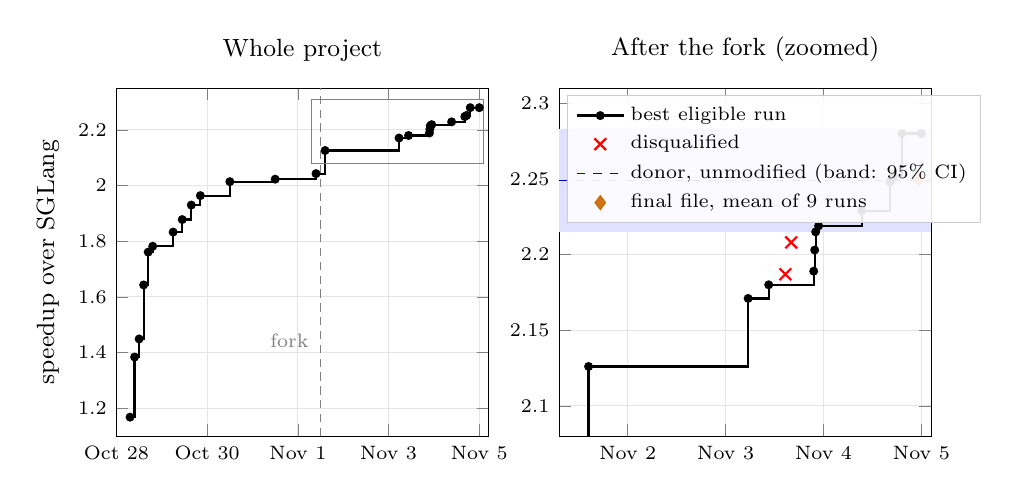
\begin{tikzpicture}
\pgfplotsset{every axis/.append style={
  height=6cm, grid=major, grid style={gray!20},
  tick label style={font=\scriptsize}, label style={font=\small},
  title style={font=\small}}}
\begin{axis}[name=left, width=0.52\linewidth,
  title={Whole project},
  xmin=0, xmax=8.2, ymin=1.1, ymax=2.35,
  xtick={0,2,4,6,8}, xticklabels={Oct 28,Oct 30,Nov 1,Nov 3,Nov 5},
  ytick={1.2,1.4,1.6,1.8,2.0,2.2}, ylabel={speedup over SGLang}]
\addplot[const plot, thick, black, mark=*, mark size=1.2pt] coordinates {
 (0.30,1.168) (0.40,1.384) (0.50,1.449) (0.60,1.643) (0.70,1.761) (0.80,1.782)
 (1.25,1.833) (1.45,1.878) (1.65,1.930) (1.85,1.964) (2.50,2.014) (3.50,2.023)
 (4.40,2.043) (4.60,2.126) (6.23,2.171) (6.44,2.180) (6.90,2.189) (6.91,2.203)
 (6.92,2.215) (6.95,2.219) (7.39,2.229) (7.68,2.248) (7.72,2.252) (7.80,2.280)
 (8.0,2.280)};
\draw[gray, densely dashed] (axis cs:4.5,1.1) -- (axis cs:4.5,2.35);
\node[font=\scriptsize, gray, anchor=north east] at (axis cs:4.45,1.5) {fork};
\draw[gray, thin] (axis cs:4.3,2.08) rectangle (axis cs:8.1,2.31);
\end{axis}
\begin{axis}[at={(left.east)}, anchor=west, xshift=0.9cm, width=0.52\linewidth,
  title={After the fork (zoomed)},
  xmin=4.3, xmax=8.1, ymin=2.08, ymax=2.31,
  xtick={5,6,7,8}, xticklabels={Nov 2,Nov 3,Nov 4,Nov 5},
  ytick={2.10,2.15,2.20,2.25,2.30},
  yticklabel style={/pgf/number format/fixed,/pgf/number format/precision=2},
  legend style={font=\scriptsize, at={(0.02,0.98)}, anchor=north west, draw=gray!40, fill=white, fill opacity=0.9, text opacity=1},
  legend cell align=left]
\addplot[fill=blue!12, draw=none, forget plot] coordinates {(4.3,2.215) (8.1,2.215) (8.1,2.283) (4.3,2.283)} -- cycle;
\addplot[const plot, thick, black, mark=*, mark size=1.2pt] coordinates {
 (4.40,2.043) (4.60,2.126) (6.23,2.171) (6.44,2.180) (6.90,2.189) (6.91,2.203)
 (6.92,2.215) (6.95,2.219) (7.39,2.229) (7.68,2.248) (7.72,2.252) (7.80,2.280)
 (8.0,2.280)};
\addlegendentry{best eligible run}
\addplot[only marks, red, mark=x, mark size=3pt, thick] coordinates {(6.61,2.187) (6.67,2.208)};
\addlegendentry{disqualified}
\addplot[dashed, blue!70!black, domain=4.3:8.1, samples=2] {2.249};
\addlegendentry{donor, unmodified (band: 95\% CI)}
\addplot[only marks, mark=diamond*, mark size=2.5pt, orange!80!black] coordinates {(7.97,2.250)};
\addlegendentry{final file, mean of 9 runs}
\end{axis}
\end{tikzpicture}
\caption{Best eligible decode-layer result over time, official judge only. Left: the
whole project; before the fork the points are our own line. Right: the boxed
region enlarged. The unmodified donor file was measured once on our account
(2.249$\times$, shaded 95\% interval); the final file's mean over nine runs falls
inside that interval. Rows on 28--31 October have dates but no recorded times and
are spread within their day.}
\label{fig:timeline}
\end{figure}

The final file ran nine times on the judge, three public runs and six private
checks. They span \num{9922.9} to \SI{10160.8}{\micro\second}, with a mean of
\SI{10054.0}{\micro\second} (2.250$\times$) and a standard deviation of 0.78\%. The best
of them, run \texttt{908cc07e43364008}, is the board row: 2.2796$\times$ with a 95\%
interval of [2.2454, 2.3139]. The judge returns a cached result for identical
bytes, so each repeat differed only in a nonce. The best run is 1.3\% faster than
the mean. That selection effect is part of the board position, and entries are
better compared by their means.

A later EAT file with one more attention build flag had a slightly lower
eight-run mean (\SI{10029.6}{\micro\second}), but none of its runs beat the row. At
22:36 Pacific on 4 November the row ranked 153rd of the layer board, which had
1{,}222 entries on 2 November. At the close the team stood 158th on the overall
board. At 18:28 Pacific the 100th-ranked entry was at 2.3028$\times$.

Per load (Table~\ref{tab:cells}), the best run's speedups are 2.574 (decode 1),
2.134 (decode 16), 1.967 (decode 32), 2.569 (verify 1), 2.169 (verify 16) and
2.330 (verify 32). Their geometric mean is 2.2796, the reported score.

The standalone boards, ranked separately, ended at 2.3893$\times$ for the
routed-expert kernel (rank 258), 2.6043$\times$ for attention and 1.5321$\times$
for the dense projections.

\section{What did not work}
\label{sec:negative}

These are the most instructive entries in the ruled-out list, with the numbers
that closed them.
\begin{description}[style=unboxed,leftmargin=0pt]
  \item[L2 prefetch of later weights during attention.] Prefetching the 34\,MB of
  o, router and unpooler weights beside attention cut the o GEMV from 7.3 to
  \SI{5.9}{\micro\second}, but the whole step got 3.5--\SI{4.1}{\micro\second} slower
  at decode 1 in the paired comparison. The prefetch traffic cost more than the hits
  saved. Several other teams reported the same in public.
  \item[Fusing across stage boundaries.] One cooperative launch for the o projection,
  the attention boundary and the pooler/router saved 0.5--\SI{1.3}{\micro\second}
  inside the process and nothing on any short load. Fusing the experts into the
  unpooler made decode 1 worse (80.7 against \SI{76.8}{\micro\second}); it replaced
  two launch boundaries with five dependent global round trips. A cooperative o
  plus boundary kernel was \SI{1.16}{\micro\second} slower in 9 of 9 rounds, from
  which we estimate a grid barrier at about \SI{1}{\micro\second}.
  \item[Using idle SMs.] The QKV GEMV launches 96 CTAs on 132 SMs. A stream-K
  version with 128 one-wave CTAs at $T = 8$--32 lost \SI{2.9}{} to
  \SI{4.0}{\micro\second} to the join alone, and the variant with no reduction lost
  too. Idle SMs were not what limited this kernel.
  \item[More concurrency in the expert kernel.] Two expert CTAs per SM lost
  7.9/\SI{8.5}{\micro\second} at decode 1, through a doubled per-CTA prologue,
  grid barrier and final work. A four-slot weight ring lost
  2.0/\SI{2.2}{\micro\second} through slower hand-off and a wider finish. A second
  N-tile, meant to avoid re-streaming weights at decode 16, lost about
  \SI{10}{\micro\second}, the third loss on that idea. In a math-only measurement at
  $T = 8$ and 32, the expert kernel's unit loop sat at an issue-throughput ceiling
  of about 0.5 warp-instructions per cycle per SM sub-partition, the same at four
  and six consumer warps. If that holds in the full kernel, the next gain there
  needs fewer instructions per weight word.
  \item[Synthetic routing.] We first chose expert-kernel variants on synthetic
  routing, where a 1--\SI{3}{\micro\second} margin on two seeds decided a
  \SI{30}{\micro\second} question. With routing skewed the way the judge's is, verify
  16 dropped 25--\SI{30}{\micro\second}.
  \item[Porting layer wins back to the standalone problems.] Projection and
  attention choices tuned inside the layer gave nothing on the standalone boards.
  Only the expert-kernel port helped there, by about 0.7\% on the box. We did not
  find out why.
\end{description}

\subsection{The routing-slack disqualification}

The rules let routing differ from the reference on near-ties. Each chosen expert
has to score within 0.05 of the reference's eighth best, and clear winners must
be kept~\cite{task}. On this GPU each distinct local expert costs the fused kernel
about \SI{6.3}{\micro\second} of weight reads. So at $T=1$ we swapped near-tied
local experts for near-tied experts on other GPUs, which this GPU then never
reads. Decode 1 got about 5 and \SI{3}{\micro\second} faster on sliding and full
layers. The file passed every correctness test. The author approved it under the
written tolerances, and it went public at \SI{10343.1}{\micro\second}, rank 355.

On 3 November at 17:45 Pacific the organizers disqualified both public runs of the
technique, and we withdrew a third. Their reason was that the change ``swaps
near-tied experts for ones on other GPUs so their weights are never read, which
changes the model's output'' and so ``goes against the spirit of the challenge''.
The row fell back to \SI{10374.6}{\micro\second} (2.180$\times$, rank 364). Every file
built on the slack file had to be rebuilt from its slack-free parent and
re-qualified. A review confirmed that the routing itself was restored, beyond
checking that the slack code was gone. Our promotion audit had also counted a
disqualified source as clean, because it read the numerical pass flags and not the
separate disqualification fields. A tolerance written to absorb a reference's
rounding is not permission to choose outputs for speed, and passing the checks is
not the same as being eligible.

\section{Process lessons}
\label{sec:lessons}

An agent team fails in ways a single engineer usually does not. Each failure
below cost real time and ended in a written rule.
\begin{description}[style=unboxed,leftmargin=0pt]
  \item[Estimated clocks.] On the last day the lead agent stamped ledger times from
  its own estimates and ran 3.5 hours ahead of the real clock. Separately, a plan
  written that morning said 11.5 hours remained when about 13.5 did. Rule: every
  ledger or schedule time comes from \texttt{date} in the same command.
  \item[Shared checkouts.] Another session's merge reset the working tree and wiped
  staged edits, which we recovered with \texttt{git fsck --dangling}. A union merge of
  a CUDA source doubled a pipeline stage-advance line, and that line was pushed.
  Rules: edit, stage, commit and push in one call; resolve source conflicts by
  hand; give every branch its own worktree.
  \item[A flag that changed the experiment.] A box script's
  \texttt{--skip-pdl8-gate} flag also turned off the expert kernel's PDL edge. With
  the flag, one change read faster in 7 of 7 pairs; without it, it read null over 3
  pairs. We built the next file without that change. Four pairs with the edge on
  later showed it 0.48/\SI{0.52}{\micro\second} faster. Rule: measure with the
  configuration the judge uses, in at least four pairs.
  \item[Rationing that narrowed the search.] The rule that ranked work by gain per
  microsecond on the cheapest loads was meant to ration judge checks. It also
  narrowed what the agents looked at, and the completion-counter fix sat in the
  excluded cells. Rule: rank engineering work by its effect on the whole score, and
  treat a feature compiled in but switched off as a lead to re-check.
  \item[Context limits.] Lane sessions reached 250{,}000--500{,}000 tokens per round
  and became slower, costlier and less reliable. Rule: each lane writes a checkpoint
  file after every step and restarts fresh after about 60 tool calls.
  \item[An async judge.] With 15--20 minute queues, a session that waited on a job
  did nothing else. Rule: submit with \texttt{--no-wait}, record the job id in the
  ledger and wait in the background.
\end{description}

\section{Discussion}

Our numbers support a plain reading. The fork's inherited design carried the
score. Our work after the fork took the file from 2.126$\times$ to a mean of
2.250$\times$, and against the unmodified donor measured on our account that gain is
zero within the judge's interval. What the work bought is the same speed with
written arguments for ordering and progress on every dependent-launch edge and on
the completion counters, which the donor shipped without. We did not show that the
donor was wrong anywhere. Whether those arguments are worth the time is a fair
question for anyone running a short competition.

Two observations may help others working at small batch on this GPU. With PDL, a
kernel boundary inside a CUDA graph cost us less than the synchronization that the
cross-stage fusions we tried put in its place. Fusion inside a stage, such as the
one-launch attention kernel, still paid. Second, a feature that someone switched
off for safety deserves a re-check against the code once the pressure is gone. Ours
held the largest single fix of the last day.

For agent-driven kernel work, the largest gains came from reading: a public file,
a top team's write-up, a disabled code path. Local tuning gave the smallest.
Measurement discipline mattered most where it was weakest. A box script measured a
different configuration than the judge, a quota rule hid the best remaining fix,
and a numerical tolerance was read as permission.

\section*{Use of AI tools}

LLM coding agents wrote most of the code and kept the experiment records:
Anthropic's Claude models through Claude Code, OpenAI Codex sessions, and the EAT
supervisor running Claude Code agents. A Claude agent drafted this report from the
repository's ledgers, and a second agent checked its claims against the sources.
The author chose the work, approved every public submission, and is responsible for
the content.

\appendix
\section{Judged layer runs}
\begin{table}[h]
\centering
\caption{Decode-layer results that set a new best, plus the disqualified runs.
Times are the board's: SGLang's fixed \SI{22620.3}{\micro\second} over the speedup.
Times marked $\sim$ are derived that way because the ledger records only the
speedup. ``check'' is a private run; DQ means disqualified. Sources:
\texttt{docs/runs-decode-layer.md} and
\texttt{docs/steering/2026-11-02-final-day-directive.md}.}
\label{tab:timeline}
\small
\begin{tabular}{lllrrr}
\toprule
date (PT) & job & change & \si{\micro\second} & speedup & rank\\
\midrule
Oct 28 & \texttt{c61c26ce} & MoE port only (check) & $\sim$\num{19366.7} & 1.168 & \\
Oct 28 & \texttt{6c9eb0ed} & + W4A16 expert GEMMs (check) & $\sim$\num{16344.1} & 1.384 & \\
Oct 28 & \texttt{b216cf4a} & cluster residual kernel (check) & $\sim$\num{15611.0} & 1.449 & \\
Oct 28 & \texttt{f23f1c81} & fused MoE, GEMV projections & $\sim$\num{13767.7} & 1.643 & \\
Oct 28 & \texttt{cc7a07e2} & one-launch attention & $\sim$\num{12845.1} & 1.761 & \\
Oct 28 & \texttt{a41ace0b} & MoE ordering repair & $\sim$\num{12693.8} & 1.782 & \\
Oct 29 & \texttt{344ae513} & judge-like MoE routing & $\sim$\num{12340.6} & 1.833 & \\
Oct 29 & \texttt{5b95c24e} & attention trimming & $\sim$\num{12044.9} & 1.878 & \\
Oct 29 & \texttt{0fae6468} & MoE schedule mode 28 & $\sim$\num{11720.4} & 1.930 & \\
Oct 29 & \texttt{9b921feb} & routing front end & $\sim$\num{11517.5} & 1.964 & \\
Oct 30 & \texttt{3fbb3ad0} & clean release, mode 47 & $\sim$\num{11231.5} & 2.014 & \\
Oct 31 & \texttt{8f2780d7} & attention port & $\sim$\num{11182.3} & 2.023 & \\
Nov 1 & \texttt{cb71acec} & residual boundary & $\sim$\num{11069.7} & 2.043 & 373\\
Nov 1 & \texttt{607eb52b} & audited fork of public file & \num{10639.4} & 2.126 & 303\\
Nov 3 05:25 & \texttt{fefd7f7b} & PDL at $T=1,16,32$ & \num{10419.9} & 2.171 & 369\\
Nov 3 10:40 & \texttt{f931abf5} & PDL at $T=8$ & \num{10374.6} & 2.180 & 364\\
Nov 3 14:40 & \texttt{9d80ae24} & routing slack (DQ) & \num{10343.1} & 2.187 & 355\\
Nov 3 16:07 & \texttt{86ed5dd3} & routing slack repeat (DQ) & \num{10243.9} & 2.208 & \\
Nov 3 21:32 & \texttt{117605d0} & clean rebuild & \num{10333.4} & 2.189 & 367\\
Nov 3 21:39 & \texttt{a7741ba2} & expert-kernel micro changes & \num{10267.5} & 2.203 & 353\\
Nov 3 22:09 & \texttt{1798d468} & $T=16$ residual on a per-row kernel & \num{10211.3} & 2.215 & 322\\
Nov 3 22:43 & \texttt{7d03f88d} & follow-up to the previous row & \num{10194.1} & 2.219 & 311\\
Nov 4 09:25 & \texttt{caed0290} & finisher in registers & \num{10146.4} & 2.229 & 308\\
Nov 4 16:20 & \texttt{40ac6a24} & expert kernel as PDL dependent & \num{10061.9} & 2.248 & \\
Nov 4 17:16 & \texttt{5dbfa4b0} & completion counters, both builds & \num{10044.3} & 2.252 & 246\\
Nov 4 19:07 & \texttt{908cc07e} & EAT cluster residual (final) & \num{9922.9} & 2.280 & 153\\
\bottomrule
\end{tabular}
\end{table}

\begin{thebibliography}{9}
\bibitem{okc} Muse Spark Open Kernel Challenge.
\url{https://openkernelchallenge.dev}, rules at
\url{https://openkernelchallenge.dev/rules}, 2026.
\bibitem{task} Muse Spark Open Kernel Challenge. Problem statement for
\texttt{muse\_decode\_layer}, \texttt{TASK.md} written by \texttt{okc init}
0.7.2, 2026.
\bibitem{repo} This work's repository, with run ledgers, profiles and the
ruled-out list. \url{https://github.com/yelgabo/okc}.
\bibitem{keell} keell0renz. Muse open kernel challenge entry and
\texttt{LESSONS.md}. \url{https://github.com/keell0renz/muse-open-kernel-challenge}, 2026.
\bibitem{vjeux} vjeux. OKC 2026 submissions.
\url{https://github.com/vjeux/okc-2026}, 2026.
\bibitem{eat} caoshiyi. EAT. \url{https://github.com/caoshiyi/EAT}, 2026.
\end{thebibliography}

\end{document}
